%!TEX TS-program = xelatex
%!TEX encoding = UTF-8 Unicode

\let\mypdfximage\pdfximage\def\pdfximage{\immediate\mypdfximage}\documentclass[14pt,a4paper]{extarticle}

\usepackage{ifthen}
\ifx\requestedLaTeXdate\undefined
\usepackage{array}
\else
\usepackage{array}[=2016-10-06]
\fi
% Packages required by doxygen
\usepackage{fixltx2e}
\usepackage{doxygen}
\usepackage{graphicx}
\usepackage[utf8x]{inputenc}
\usepackage[ukrainian]{babel}
\usepackage{makeidx}
\PassOptionsToPackage{warn}{textcomp}
\usepackage{textcomp}
\usepackage[nointegrals]{wasysym}
\usepackage{ifxetex}

\usepackage{mathtools} % Mathematical tools to use with amsmath
%\usepackage{amsfonts} % TeX fonts from the American Mathematical Society
\usepackage{ifxetex}
\usepackage{indentfirst} % Indent first paragraph after section header
\ifxetex
  \usepackage{mathspec} % Specify arbitrary fonts for mathematics in XeTeX
  \usepackage{fontspec} % Advanced font selection in XeLaTeX and LuaLaTeX
  %\usepackage{polyglossia} % Multilingual support for XeLaTeX
\else
  %\usepackage[utf8x]{inputenc}
  \usepackage[T1]{fontenc}
  \usepackage[ukrainian]{babel}
\fi
\usepackage[
  left=2.5cm,right=1.5cm,top=1.5cm,bottom=1.5cm,
  headheight=5mm,headsep=5mm,includehead
]{geometry} % Flexible and complete interface to document dimensions
\usepackage{makeidx} % Standard LaTeX package for creating indexes
%\usepackage[
%  colorlinks=true, allcolors=black,
%]{hyperref} % Extensive support for hypertext in LaTeX
\usepackage{titlesec} % Select alternative section titles
%\usepackage{array} % Extending the array and tabular environments
\usepackage{amsthm} % Typesetting theorems (AMS style)
%\usepackage{mathrsfs} % Support for using RSFS fonts in maths
%\usepackage{amssymb}

%\usepackage{cprotect}% http://ctan.org/pkg/cprotect
%\usepackage{listings} % Typeset source code listings using LaTeX
%\usepackage{minted}
\usepackage{fancyhdr}
\usepackage{ulem}
%\usepackage{multicol}
\usepackage[nottoc]{tocbibind}
%\usepackage{longtable}
%\usepackage{pgfplots} % Create normal/logarithmic plots !slow
\usepackage{titletoc}
\usepackage{pgf}
%\usepackage{tikz}
\usepackage[section]{placeins}
\usepackage[labelsep=period,bf,textfont=bf]{caption}
%\usepackage{pst-node, pst-plot, auto-pst-pdf}
\usepackage{setspace}

% latex
\pagestyle{myheadings}

\ifxetex
  % mathspec
  \setmathsfont(Digits,Latin,Greek){Times New Roman}

  % fontspe
  \defaultfontfeatures{Mapping=tex-text}
  \setmainfont{Times New Roman}
  \newfontfamily\cyrillicfont{Times New Roman}
  %\setmonofont[Mapping=tex-text]{Fantasque Sans Mono}
  %\newfontfamily\cyrillicfontsf[Script=Cyrillic]{Fantasque Sans Mono}
  %\newfontfamily\cyrillicfonttt[Script=Cyrillic]{Fantasque Sans Mono}

  % polyglossia
  %\setdefaultlanguage{ukrainian}
\fi

% titlesec
\titleformat{\section}
  {\newpage\normalfont\Large\bfseries\centering\MakeUppercase}{\thesection. }{0pt}{}
\titleformat{\subsection}
  {\normalfont\large\bfseries\centering}{\thesubsection. }{0pt}{}
\titleformat{\subsubsection}
  {\normalfont\bfseries}{\thesubsubsection. }{0pt}{}
%\titlespacing\section{0pt}{0pt plus 0pt minus 0pt}{0pt plus 0pt minus 0pt}
%\titlespacing\subsection{0pt}{0pt plus 0pt minus 0pt}{0pt plus 0pt minus 0pt}
%\titlespacing\subsubsection{0pt}{0pt plus 0pt minus 0pt}{0pt plus 0pt minus 0pt}

% array
\def\arraystretch{1.5}

% amsthm
\newtheorem{theorem}{Теорема}[section]
\theoremstyle{definition}
\newtheorem{definition}{Визначення}[section]

\linespread{1.5}
\setlength{\parindent}{1cm}
\setlength{\parskip}{0.5\baselineskip}%
\bibliographystyle{plain}
%\dottedcontents{section}[1em]{}{1.5em}{1pc}
%\dottedcontents{subsection}[2.5em]{}{2em}{1pc}
%\titlecontents*{section}[0cm]{\small}{\thecontentslabel. \uppercase}{\uppercase}{ \titlerule*[1pc]{.}\contentspage\\}[][]
\titlecontents*{subsection}[0cm]{\small}{\hspace*{1cm}\thecontentslabel. }{}{ \titlerule*[1pc]{.}\contentspage\\}[][]
\titlecontents*{subsubsection}[0cm]{\small}{\hspace*{2cm}\thecontentslabel. }{}{ \titlerule*[1pc]{.}\contentspage\\}[][]

\makeatletter
\def\@maketitle{%
  \newpage%
  \linespread{1}\rmfamily%
  \begin{center}%
    {\bfseries ДНІПРОВСЬКИЙ НАЦІОНАЛЬНИЙ УНІВЕРСИТЕТ \\%
    ІМЕНІ ОЛЕСЯ ГОНЧАРА \\%
    ФАКУЛЬТЕТ ПРИКЛАДНОЇ МАТЕМАТИКИ \\%
    КАФЕДРА КОМП'ЮТЕРНИХ ТЕХНОЛОГІЙ \\}%
  \end{center}%
  \vspace*{5pt}%
  {\@title \par}%
  \hfill \break%
  \begin{flushright}%
    {\linespread{1}%
      \begin{tabular}[b]{p{8cm}}%
        \@author%
      \end{tabular}\par}%
  \end{flushright}
  \vspace*{\fill}
  {\centering м. Дніпро, 2021 р.\par}}
\makeatother

\makeatletter
%\renewcommand{\[}{\begin{dmath*}[compact]}
%\renewcommand{\]}{\end{dmath*}}
%\newcommand{\bdg}{\begin{dgroup*}}
%\newcommand{\edg}{\end{dgroup*}}
%\newcommand{\bdg}{}
%\newcommand{\edg}{}
\renewcommand{\[}{\begin{singlespace}\begin{equation*}}
\renewcommand{\]}{\end{equation*}\end{singlespace}}
\newcommand{\be}{\begin{enumerate}}
\newcommand{\ee}{\end{enumerate}}
\newcommand{\ds}{\displaystyle}
\newcommand{\sep}{ , \ \allowbreak }
\newcommand{\ivr}{\rule[-2.25ex]{0pt}{6ex}}
\newcommand\fr[2]{\dfrac{#1}{#2}}
\newcommand{\sigmalgebra}{\text{\textcircled{$\sigma$}}}
\newcommand\uname[3]{\parbox[b][\height][b]{#1}{\tiny\underline{\normalsize\parbox[c][4mm][t]{#1}{\makebox[#1]{#2}}}\newline\makebox[#1]{(#3)}}}
\newcommand\eeq[1][]{\stackrel{\mathclap{\normalfont\mbox{#1}}}{=}}
\renewcommand{\@biblabel}[1]{#1.}
\addto\captionsukrainian{\renewcommand{\refname}{СПИСОК ВИКОРИСТАНОЇ ЛІТЕРАТУРИ}}
\addto\captionsukrainian{\renewcommand{\figurename}{Рис.}}
\makeatother

\protect\setcounter{tocdepth}{1}

\title{\begin{center}
    {\bfseries ЗВІТ\\
    З ПРЕДДИПЛОМНОЇ ПРАКТИКИ}\\
  \end{center}
  Освітньо-професійна програма: Комп'ютерне моделювання та технології програмування\\[3mm]
  Спеціальність: 113 Прикладна математика\\[3mm]
  Галузь знань: 11 Математика і статистика\\[3mm]
  Рівень вищої освіти: перший (бакалаврський)}
\author{Cтудента 4 курсу групи ПА–17–2 \newline%
  \uname{8cm}{Панасенко Єгор Сергійович}{прізвище та ініціали}\newline\newline
  Керівник: \uline{канд. фіз.-мат. наук\hfill} \newline%
  \uname{8cm}{Степанова Наталія Іванівна}{посада, вчене звання, науковий ступінь, прізвище та ініціали} \newline\newline
  Кількість балів: \uline{\hfill}\newline\newline
  Національна шкала: \uline{\hfill}\newline\\
  \bgroup
  %\def\arraystretch{1}
  \begin{tabular}[b]{@{}p{3cm}@{}p{5cm}@{}}
    \multicolumn{2}{l}{Члени комісії:}\\
    \uname{3cm}{\hfill}{підпис}
      & \uname{5cm}{Зайцева Т.А.}{прізвище та ініціали} \\
    \uname{3cm}{\hfill}{підпис}
      & \uname{5cm}{Сердюк М.Є.}{прізвище та ініціали} \\
    \uname{3cm}{\hfill}{підпис}
      & \uname{5cm}{Лисиця Н.М.}{прізвище та ініціали} \\
  \end{tabular}\egroup}
\date{}

% Hyperlinks (required, but should be loaded last)
\ifpdf
  \usepackage[pdftex,
  colorlinks=true, allcolors=black,]{hyperref}
\else
  \ifxetex
    \usepackage[
  colorlinks=true, allcolors=black,]{hyperref}
  \else
    \usepackage[ps2pdf,
  colorlinks=true, allcolors=black,]{hyperref}
  \fi
\fi

%\newcommand{\+}{\discretionary{\mbox{\scriptsize$\hookleftarrow$}}{}{}}

\hypersetup{%
  colorlinks=true,%
  linkcolor=blue,%
  citecolor=blue,%
  unicode%
}

\begin{document}
\stepcounter{tocdepth}
\sloppy % Stretches spaces to correct align of text
\allowdisplaybreaks % Breaks equations between pages
\maketitle
\thispagestyle{fancy}
\fancyhf{}% Clear all headers/footers
\renewcommand{\headrulewidth}{0pt}% No header rule
\renewcommand{\footrulewidth}{0pt}% No footer rule

{
\titlecontents*{section}[0pt]{\small}{\thecontentslabel. \uppercase}{\uppercase}{ \titlerule*[1pc]{.}\contentspage\\}[][]
\tableofcontents
}
\section*{ВСТУП}
\addcontentsline{toc}{section}{ВСТУП}
Створення просторових моделей об'єктів виконується сьогодні у багатьох галузях науки і промисловості, таких як архітектура, медицина, будівництво, дизайн. Особливої уваги заслуговують також засоби подання динамічних 3D-об'єктів, які  широко використовуються у кінематографі, індустрії комп'ютерних ігор.

У сучасному світі спостерігається неймовірний приріст потужності обчислювальної техніки і розробники систем віртуальної реальності,  комп'ютерних ігор намагаються використати цю потужність якомога ефективніше з метою отримання графіки, найбільш схожої на реальний світ.

Для досягнення максимального задоволення користувачів розробники також створюють велику кількість окремих об'єктів та приголомшливих ефектів, що супроводжується значним споживання дискового простору й оперативної пам'яті. Тому завжди є актуальними питання розробки більш ефективних методів моделювання об'єктів складної форми, які б використовували менше обчислювальних ресурсів.

Які можливості сьогодні мають розробники інтерактивних програмних продуктів для зберігання об'єктів? По-перше, майже двадцять років тому, коли потужність процесорів достатньо зросла, щоб швидко виконувати великі об'єми обчислень, було розроблено векторний формат SVG. Для побудови зображень формат використовує криві Безьє, які є окремим випадком B-сплайнів. Сьогодні формат SVG є поширеним, він підтримується всіма сучасними браузерами для настільних і мобільних пристроїв.

Формат SVG дозволяє зберігати як статичну, так і анімовану двовимірну графіку. Якщо розглядати використання SVG формату у інтерактивних системах, зокрема у комп'ютерних іграх, дуже цікавою є можливість закріплення за об'єктом у даному форматі обробника подій, що дає користувачеві можливість керувати зображенням: міняти його форму, пересувати.
Крім того, векторним форматам притаманні гарна масштабованість й незначне використання дискового простору за умови, що зображення складається з невеликої кількості простих елементів, що також сприяє популярності SVG формату у розробників інтерактивних графічних додатків. 

З іншого боку, SVG як і всі векторні формати, має також і недоліки: у порівнянні з растровими аналогами побудова SVG-зображення потребує більше процесорного часу, а зображення, що складаються з великої кількості дрібних деталей, починають вимагати більше дискового простору ніж аналогічні растрові. 

Також суттєвим обмеженням для використання формату SVG у індустрії комп'ютерних ігор є те, що він не підтримує опис тривимірної графіки.

У тривимірному просторі найбільш розповсюдженим форматом є OBJ – простий і гнучкий формат, що дозволяє створювати об'єкти за допомогою різних способів, у тому числі з використанням кривих Безьє і B-сплайнів.
 
Таким чином на даний час вже існують формати, які дозволяють зберігати окремі об'єкти компактно, забезпечувати їх легку масштабованість.

Але у реальному ігровому процесі, де об'єкти мають досить складні форми,  постійно взаємодіють один з одним, а сцени є досить насиченими, виникає проблема: як найбільш просто зробити опис об'єктів і забезпечити їх подальшу динаміку з найменшим навантаженням на комп'ютерну систему?

\section*{ПОСТАНОВКА ЗАДАЧІ}
\addcontentsline{toc}{section}{ПОСТАНОВКА ЗАДАЧІ}

Метою цієї роботи є розробка програмного забезпечення для генерація та відображення 3D-моделей об'єктів у комп'ютерних іграх з використанням сплайнів у режимі реального часу. У загальному випадку розглядаються 3D-моделі об'єктів створені за допомогою поверхонь Безьє. Для досягнення поставленої мети були поставлені наступні задачі:

\begin{itemize}
\item розширити функціонал розробленого програмного забезпечення, розробленого у курсовій роботі, загалом додати можливість динамічно завантажувати моделі, змінювати деталізацію.
\item зробити програмне забезпечення придатним для компіляції та роботи у різних операційних системах, загалом Linux та Windows
\item розробити шйедер для генерації 3D-моделі за допомогою відеокарти.
\item написати документацію до програмного забезпечення.
\end{itemize}

\section{Аналітичний огляд літературних джерел}

\subsection{Математичні моделі поверхонь та об'єктів}

Комп’'терна графіка пропонує сьогодні різні засоби моделювання просторових форм і об'єктів. Геометричне моделювання - це математичний опис об'єктів у просторі певними атрибутами: координатами, розмірами, формою. При відображенні геометричних об'єктів потрібно враховувати також їх просторове розташування і поведінку: переміщення, повороти відносно координатних осей (шість ступенів свободи), зіткнення з перешкодами або іншими об'єктами. Крім того для отримання образів просторових форм на площині екрану необхідно використовувати ще одне геометричне перетворення - проеціювання. 

\subsubsection{Математичний опис моделей поверхонь та об’єктів}

У комп'ютерній графіці прийнята така класифікація моделей поверхонь і об'єктів:
\begin{itemize}
\item Каркасні - на екрані візуалізуються не всі точки поверхні, а лише невелика їх кількість, достатня, щоб передати характер поверхні. Пари точок утворюють  систему ліній і формують каркас моделі;
\item Точкові - на екрані відображаються точки з відповідним забарвленням;
\item Кінематичні - поверхня будується неперервним рухом у просторі лінії по заданій траєкторії;
\item Кусочні – поверхня складається з окремих фрагментів,  при обмеженому наборі даних у поверхні присутні розриви і злами;
\item Сплайнові – моделі використовуються для побудови гладких поверхонь на основі обчислення координат за допомогою розв'язання систем лінійних алгебраїчних рівнянь;
\item Фрактальні – при побудові поверхні використовується властивість об'єктів до самоподібності в залежності від масштабу;
\item Графічні - використовуються у разі, якщо не можливо виділити певний закон для побудови і поверхня заповнюється деякими дискретними елементами.
\end{itemize}

У загальному випадку не можна стверджувати, що одна математична модель краща за іншу. Так, наприклад, каркасна модель зручна для виконання швидкої візуалізації поверхні, кінематична підходить для  об'єктів з природною симетрією, графічна дає більш реалістичне уявлення про об'єкт.  Тому необхідно обирати математичну модель з урахуванням потрібного ступеня реалістичності, обчислювальних можливостей комп'ютерної системи, особливостей задачі, для якої застосовується моделювання об'єктів.

\subsubsection{Опис розташування об'єктів у сцені}

Сцена у комп'ютерній графіці - це сукупність об'єктів, які підлягають відображенню, описана за допомогою деякої математичної моделі. Візуалізацією називають процес перетворення математичної моделі сцени у вигляд, придатний для показу на наявних пристроях виведення.

Для подання об'єктів сцени у графіці використовують декілька координатних систем: об'єктну (жорстко зв'язана з об'єктом), світову (нерухома система, призначена для визначення взаємного розташування всіх об'єктів сцени), видову (система спостерігача, визначає напрямок камери і ракурс показу).

Для здійснення переходу від однієї координатної системи до іншої використовуються матриці базових геометричних перетворень (зсуву, обертання, масштабування). Складні перетворення визначаються шляхом перемноження матриць відповідних елементарних перетворень між собою. Таким чином спочатку відбувається перехід від об'єктної системи координат до світової, а потім зі світової до видової.

Після отримання видових координат об'єктів сцени виконується проектування сцени на екранну площину. Для цього використовується матриця проективного перетворення (паралельне або центральне проектування), яка дає змогу отримати екранні (двовимірні) координати об'єктів сцени. Третя видова координата зазвичай зберігається; з її допомогою визначають взаємне розташування об'єктів сцени за глибиною.

На останньому кроці відбувається перетворення координат об’єктів з урахуванням особливостей системи графічного виводу.

\subsection{Дослідження математичних моделей складних об'єктів}

Для подальшої програмної реалізації серед існуючих математичних моделей поверхонь об'єктів було обрано поверхню Безьє, яка є частинним випадком B-сплайнів.

\subsubsection{Сплайни і сплайн-інтерполяція}

Існує досить велика кількість геометричних конструкцій, які називають сплайнами. Наприклад, експоненціальні (напружені) сплайни, тригонометричні, раціональні сплайни. У комп'ютерній графіці найбільш широке застосування знайшли кубічні сплайни та метод інтерполяції кубічними сплайнами.

Особливість сплайн-інтерполяції полягає в тому, що сплайнова крива складається з кількох поліномів третього ступеня, а їх кількість дорівнює кількості інтервалів, всередині яких ми виконуємо інтерполяцію. Гладкість побудованої інтерполяційної кривої забезпечується безперервністю першої похідної на всьому інтервалі інтерполяції.

Розглянемо загальний випадок спланової кривої. Нехай у тривимірному просторі існують вектори $u_i = [x_i\ y_i\ z_i], i=\overline{0,n}$, ці вектори визначають вузлові точки сплайнової кривої. Будемо вважати, що вузлові точки пронумеровані у порядку з’єднання кривої.


Параметричне подання сплайнової кривої має вигляд:
\[\left\{\begin{array}{l}
x_i(t)=s_{3x_i}t^3+s_{2x_i}t^2+s_{0x_i}t+s_{1x_i}\\
y_i(t)=s_{3y_i}t^3+s_{2y_i}t^2+s_{0y_i}t+s_{1y_i}\\
z_i(t)=s_{3z_i}t^3+s_{2z_i}t^2+s_{0z_i}t+s_{1z_i}\\
\end{array}\right.\]
або у  векторній формі:
\[\left\{\begin{array}{l}
p_i(t)=[t^3\quad t^2\quad t\quad 1]\ S_i\\
\forall t \in [0, d_i],\ i = \overline{0,n}
\end{array}\right.\text{, де }S_i=\left[\begin{matrix}
s_{3x_i} && s_{3y_i} && s_{3z_i} \\
s_{2x_i} && s_{2y_i} && s_{2z_i} \\
s_{1x_i} && s_{1y_i} && s_{1z_i} \\
s_{0x_i} && s_{0y_i} && s_{0z_i} \\
\end{matrix}\right]\]

З урахуванням властивостей сплайнів будується система лінійних алгебраїчних рівнянь відносно невідомих коефіцієнтів сплайну:
\[QS=U \to S=Q^{-1}U\]
де $Q\in R^{4n\times4n}$ - матриця яка задає необхідні умови для системи, 
$S=\left[\begin{array}{c}S_1\\\dots\\\S_n\end{array}\right]\in R^{4n\times3}, U \in R^{4n\times3}$

\subsubsection{Крива Безьє}

Окремим випадком сплайнів є крива Безьє. Кубічну криву Безьє можна побудувати з використанням чотирьох опорних точок $P_i, i=\overline{0,3}$. У параметричному вигляді отримаємо:
\[B(t)=(1-t)^3P_0+t(1-t)^2P_1+t^2(1-t)P_2+t^3P_3\]
де t -- параметр, $t \in [0,1]$

Розглянемо графічний спосіб побудови кривої Безьє із застосуванням алгоритму де Кастельє (рис. $\cite{fig:bezier_curve}$).

\begin{figure}[!htb]
    \centering
    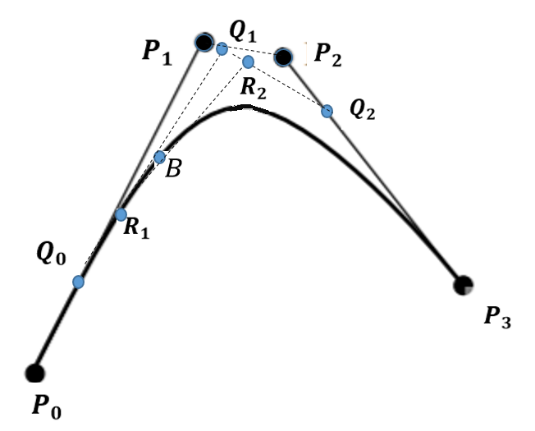
\includegraphics[width=0.5\textwidth]{bezier-curve.png}
    \caption{Побудова кривої Безьє}\label{fig:bezier_curve}
\end{figure}

Для отримання точки кривої, яка відповідає, наприклад, значенню параметра $t=0.25$ потрібно відкладасти $0.25$ шляху на відрізках $P_iP_{i+1}$. В результаті отримаємо точки $Q_{j}, j=\overline{0,2}$, на наступному кроці зробимо теж саме і отримаємо $R_0$ та $R_1$.У такий спосіб чином ми отримали дотичну до кривої, ця властивість буде використана для побудови нормалі у поверхні кривої Безьє. І знову прокладемо $0.25$ шляху на відрізку $R_0R_1$ отримаємо нашу точку $B$, яка знаходиться на кривій. Якщо ми будемо послідовно обирати $t$, наприклад з кроком $0.1$, та з'єднувати у відрізки, то ми отримаємо ламану. Зі зменшенням кроку ламана буде ставати все більш схожою на криву. Таким чином можна підібрати такий крок, при якому на екрані комп'ютера буде відображатися крива.

Крива Безьє задається формулою:
\[B(t)=\sum_{i=0}^n P_i b_{i,n}(t)\]
де $P_i$ - контрольні точки, а $b_{k,n}(t)$ - поліноми Бернштейна, базисні функції кривої Безьє.
\[b_{k,n}(t)=C_i^nt^k(1-t)^{n-k}\]
де $C_i^n$ число поєднань з $n$ по $k$
\[C_i^n=\frac{n!}{k!(n-k)!}\]

Побудуємо формулу кубічної кривої Безьє:
\[B(t)=(1-t)^3P_0+t(1-t)^2P_1+t^2(1-t)P_2+t^3P_3\]

Цю формулу можна отримати побудувавши криву графічним способом. Прокласти шлях від однієї контрольної точки до іншої можна таким чином $(1-t)P_i+tP_{i+1}$, якщо ми послідовно проробимо ті самі кроки, що і у графічному будуванні, отримаємо:
\begin{align*}
B(t)=&t (t ((1 - t) P_{2} + t P_{3}) + (1 - t) ((1 - t) P_{1} + t P_{2})) +\\
&+(1 - t) (t ((1 - t) P_{1} + t P_{2}) + (1 - t) ((1 - t) P_{0} + t P_{1}))
\end{align*}

Спростимо формулу:
\begin{equation}
\label{eq:bezier_curve}
B(t) = -t^3P_0+3t^3P_1-3t^3P_2+t^3P_3 + 3t^2P_0-6t^2P_1+3t^2P_2 - 3tP_0+3tP_1 + P_0
\end{equation}

Тепер ми можемо записати формулу у матричному вигляді:
\[B(t)=[t^3\quad t^2\quad t\quad 1]\left[\begin{matrix}
-1 &  3 & -3 & 1 \\
 3 & -6 &  3 & 0 \\
-3 &  3 &  0 & 0 \\
 1 &  0 &  0 & 0 \\
\end{matrix}\right]\left[\begin{matrix}
P_0 \\ P_1 \\ P_2 \\ P_3 \\
\end{matrix}\right]\]
aбо нехай $P_i = [p_{ix}\ p_{iy}\ p_{iz}\ 1]$
\[B(t)=[t^3\quad t^2\quad t\quad 1]\left[\begin{matrix}
-1 &  3 & -3 & 1 \\
 3 & -6 &  3 & 0 \\
-3 &  3 &  0 & 0 \\
 1 &  0 &  0 & 0 \\
\end{matrix}\right]\left[\begin{matrix}
p_{0x} & p_{0y} & p_{0z} & 1 \\
p_{1x} & p_{1y} & p_{1z} & 1 \\
p_{2x} & p_{2y} & p_{2z} & 1 \\
p_{3x} & p_{3y} & p_{3z} & 1 \\
\end{matrix}\right]\]

Враховуючи що на сучасних комп'ютерах завдяки кешуванню рядків, то множити матрицю на вектор швидше ніж вектор на матрицю, то більш оптимальною формулою буде: 
\[B(t)=\left[\begin{matrix}
p_{0x} & p_{0y} & p_{0z} & 1 \\
p_{1x} & p_{1y} & p_{1z} & 1 \\
p_{2x} & p_{2y} & p_{2z} & 1 \\
p_{3x} & p_{3y} & p_{3z} & 1 \\
\end{matrix}\right]^T\left[\begin{matrix}
-1 &  3 & -3 & 1 \\
 3 & -6 &  3 & 0 \\
-3 &  3 &  0 & 0 \\
 1 &  0 &  0 & 0 \\
\end{matrix}\right]\left[\begin{matrix}t^3\\t^2\\t\\1\end{matrix}\right]\]

Тепер знайдемо похідну до вираження (\ref{eq:bezier_curve}), для того щоб знайти дотичну, отримаємо:
\begin{equation}
B(t) = -3t^2P_0+9t^2P_1-9t^2P_2+3*t^2P_3 + 6tP_0-12tP_1+6tP_2 - 3P_0+3P_1
\end{equation}

Запишемо у матричному вигляді:
\[B(t)=\left[\begin{matrix}
p_{0x} & p_{0y} & p_{0z} & 1 \\
p_{1x} & p_{1y} & p_{1z} & 1 \\
p_{2x} & p_{2y} & p_{2z} & 1 \\
p_{3x} & p_{3y} & p_{3z} & 1 \\
\end{matrix}\right]^T\left[\begin{matrix}
 0 &   0 &  0 & 0 \\
-3 &   9 & -9 & 0 \\
 6 & -12 &  6 & 0 \\
-3 &   3 &  0 & 0 \\
\end{matrix}\right]^T\left[\begin{matrix}t^3\\t^2\\t\\1\end{matrix}\right]\]

Властивості кривої Безьє:
\begin{itemize}
\item неперервність заповнення сегменту між початковою та кінцевою точками,
\item крива завжди знаходитися у фігурі утвореній контрольними точками, у кубічній кривій це буде деякий чотирикутник, цю властивість можна використати для того щоб перевірити чи не перетинаються дві криві на початковому етапі,
\item якщо контрольні точки знаходяться на одній прямій, то утворюється пряма лінія,
\item крива симетрична, тобто якщо переставити вектор контрольних точок у зворотьому порядку, то отримаємо ту саму форму,
\item крива афінно інваріантна,
\item зміна однієї контрольної точки приводить до зміни всієї кривої,
\item будь який сегмент кривої є крива Безьє.
\end{itemize}

\subsubsection{Поверхня Безьє}

Як і крива Безьє, поверхня Безьє визначається набором контрольних точок. Розглянемо графічний спосіб побудови кубічної поверхні Безьє з 16 контрольними точками (рис. \cite{fig:bezier-surface}). 

\begin{figure}[!htb]
    \centering
    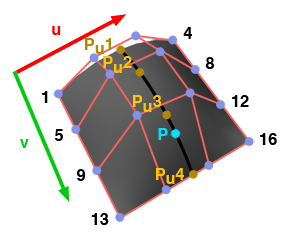
\includegraphics[width=0.5\textwidth]{bezier-surface.png}
    \caption{Побудова поверхні Безьє}\label{fig:bezier-surface}
\end{figure}

Спочатку будуємо 4 кубічні криві Безьє через контрольні точки 1-4, 5-8, 9-12, 13-16 використовуючи дійсне число $v$, далі використовуючи точки відповідних $v$ на отриманих кривих як контрольні точки наступної кривої будуємо наступну криву використовуючи дійсне число $u$, таким чином ми отримаємо поверхню побудованої з багатьох кривих, причому як ми все знаємо відрізок отриманий в останньому кроці при побудові кривої це дотична, якщо ми побудуємо поверхню будуючи криві по контрольним точкам 1, 5, 9, 13 і так далі до 4, 8, 12, 16, то ми отримаємо ще одну дотичну, але в деякому іншому напрямку, і якщо ми знайдемо векторний добуток отриманих дотичних, ми отримаємо нормаль до поверхні у даній точці.

Поверхня Безьє задається формулою:
\[p(u,v)=\sum_{i=0}^n\sum_{j=0}^n b_{i,n}(u) b_{j,n}(v) P_{ij}\]

В комп'ютерній графіці поверхні Безьє використовують для подання гладких поверхонь. Вони досить компактні, ними легко маніпулювати, вони мають гарні властивості безперервності. Крім того, такі канонічні поверхні, як сфери і циліндри, можна добре апроксимувати невеликим числом кубічних поверхонь Безьє.

\section{Розробка програмного забезпечення щодо створення і редагування гладких об'єктів}

На початку розробки графічного додатку розробник повинен визначитися, з якого рівня починати писати власний програмний код. Програмуванням на рівні графічного обладнання, як правило, займаються лише його виробники. Графічна бібліотека, яка реалізує певний стандарт абстрагування від обладнання, безпосередньо взаємодіє з драйвером. Стандартами абстрагування є, наприклад, бібліотеки OpenGL (відкрита графічна бібліотека для настільних комп'ютерів під керуванням різних ОС), Direct3D (призначена для різних ЕОМ під управлінням Windows і Windows Phone), Metal (для мобільних пристроїв під керуванням iOS). \cite{ryabin}

У даній роботі для розробки програмного продукту обрано крос-платформовий програмний інтерфейс OpenGL, що забезпечує незалежність програмного додатку від операційної системи.

\subsection{Бібліотека Visualization Library}

У ході роботи було знайдено таку біблиотеку, як Visualization Library. Ця біблиотека написана на мові C++ і може використовуватись для графіки у 2D або 3D. Вона дозволяє моделювати різні види поверхонь, фрактали, та багато іншого. Проаналізувавши можливості використання бібліотеки було отримано такі висновки:

\begin{itemize}
\item Бібліотека написана на мові C++ та з використанням виключень, таким чином це робить неможливим її використання іншими мовами програмування.
\item Бібліотека самостійно реалізує свою матрицю та вектор, таким чином закривають можливість оптимізувати операції над матрицями. Більш того бібліотека не  використовує команди SSE, які дають приріст у швидкості, як це зроблено у бібліотеці CGLM.
\item Бібліотека вже не підтримується розробниками, останній внесення змін у код було 20 лютого 2020 року, у порівнянні з бібліотекою CGLM, яка активно розвивається.
\item Якщо подивитися на реалізацію кривих Безьє, то ми побачимо, що бібліотека не використовує матричний спосіб отримання вершин з поверхні Безьє, таким чином ми знову не можемо використати оптимізацію за допомогою команд SSE.
\item Також перерірено спосіб знаходження нормалей для поверхні, біблиотека знаходить нормалі по отриманим трикутникам при будуванні поверхні, хоча для поверхні Безьє існує значно швидший та дешевший спосіб знаходження нормалі, цей спосіб будується на знаходження похідних до кривої Безьє з різних сторін.
\end{itemize}

\section{Вимоги до розробленого програмного забезпечення}

Для розробки програмного забезпечення висунуто такі вимоги:
\begin{itemize}
\item Програмне забезпечення повинно мати відкритий вихідний код та ліцензію вільного програмного забезпечення.

Це дозволить будь якому досвідченому користувачу зкомпілювати програмне забезпечення під будь яку платформу та операційну систему, або навіть дасть можливість модифікувати код під свої потреби.

Також ліцензія повинна бути сумісна з ліцензіями використаних бібліотек. Загалом були використані бібліотеки CGLM, ImGui, GLFW, EASTL та прогрмний інтерфейс OpenGL. Перші біблиотеки CGLM та ImGui використовують ліцензію MIT, бібліотека GLFW використовує ліцензію ZLib, а EASTL -- ліцензію BSD. А програмний інтерфейс OpenGL має ліцензію подібну до ліцензії BSD. Усі ці ліцензії є сумісними з ліцензією LGPLv3, яка є подібною до GPL, але дозволяє використовувати програмне забезпечення у пропріетарних проектах.

\item Програмне забезпечення повинно працювати у режимі реального часу.

Саме таким чином було вибрано мову C++ та бібліотеку CGLM, які дозволяють досягти найбільшої швидкості роботи програми у порівнянні з іншими мовами програмування, причому практично не знижуючи швидкості розробки коду. Більш того CGLM автоматично компілюється з використанням SSE команд, якщо є така можливість, що ще дає приріст у швидкості.

\item Програмне забезпечення повинно дати можливість використання бібліотеки якомога більшому колу розробників.

Саме тому було обрано мову програмування C++ та бібліотеку EASTL, яка на відміну від стандартної бібліотеки STL дозволяє розробляти без використання виключень. Таким чином за допомогою інструментів можна на основі цього програмного забезпечення згенерувати C код, який у подальшому можна обернути у більшість мов програмування і таким чином програмне забезпечення зможуть використати і розробники, які не знають C++, але знають деяку іншу мову програмування.

\item Програмне забезпечення повинно бути якомога простим та легким, та залежати від простих та легких бібліотек.

Програмне забезпечення повинно розроблятися по принципу KISS (акронім для ``Keep it simple, stupid''), що означає що проектування повинно бути якомога простішим. Таким чином можна уникнути багатьох помилок пов'язані з тим що неможливо розробник не може охопити структуру вихідного коду складного програмного забезпечення, а також таке програмне забезпечення має дуже малий розмір зкомпільованої програми, що підвищує легкість розповсюдження.  А також саме тому було вибрано саме такий набір бібліотек, а загалом графічну бібліотеку ImGui, яка має досить невеликий обсяг коду, приблизно 30 тисяч строк коду разом з коментарями.
\end{itemize}


\section{Опис програмного забезпечення}

Було розроблено програмне забезпечення на мові C++ для моделювання поверхні Безьє за допомогою програмного інтерфейсу OpenGL, що використовується для відображення 2D та 3D векторної графіки на екран, основна особливість, чому була вибрано саме OpenGL це те що інтерфейс має вільну ліцензію подібну до BSD, її підтримують більшість оперативних систем та інтерфейс на мові Сі. Також були використані бібліотеки:

\begin{itemize}
\item CGLM - математична бібліотека написана на мові Cі. Використовує ліцензію MIT.

У программі загалом використовується для афінних перетворень та арифметичними операціями між матрицями. За замовчанням використовує команди SSE, що дозволяють прискорити швидкість обчислення завдяки повному виковистанню особливостей обчислення процесорів.

\item ImGui - бібліотека для графічного інтерфейсу написана на мові C++. Використовує ліцензію MIT.

Бібліотека має невелику кодову базу порівняно з аналогічними графічними бібліотеками та фреймворками, такими як GTK або QT, та дозволяє створювати динамічні віджети.

\item GLFW - бібліотека для відображення вікна з OpenGL та обробки вводу. Використовує ліцензію ZLib.

\item EASTL - бібліотека для заміни стандартного STL. Використовує ліцензію BSD.

Бібліотека EASTL дозволяє замінити стандартну бібліотеку STL для того щоб уникнути виключень, що не оброблюється деякими мовами програмування. Також бібліотека цікава тим що вона реалізує оптимізовані версії контейнерів, що мають такий же самий інтерфейс, що і звичайні контейнери.
\end{itemize}

Код програмного забезпечення складається з таких компонентів:
\begin{itemize}
\item Вихідний код програми, який зберігається у директорії ``osdo''. Тут знаходиться бібліотека ``osdo'', яка не використовує STL, таким чином її можна використовувати іншими мовами програмування. Загалом тут знаходяться файли заголовків з розширенням ``.h'' та з реалізацією з розширенням ``.cpp'', кожен файл заголовків у цій директорії утворює окремий клас.
\item Вихідний код програми, який зберігається у директорії ``druidengine''. Тут знаходиться інтерфейс програми, так як деякі компоненти ImGui, такі як файловий менеджер, використовує STL, це унеможливлює використання іншими мовами програмування, хоча це і не потрібно, так как інтерфейс програми не потібен для розробки. Загалом тут знаходяться файли заголовків з розширенням ``.h'' та з реалізацією з розширенням ``.cpp'', кожен файл заголовків у цій директорії утворює окремий клас.
\item Ресурси програми, які зберігаються у директорії ``res'' (скорочено ``resource''). Тут знаходяться шейдери та тестові моделі чайнику, моделі машини та деякої еліпсоподібної моделі.
\item Файл з правилами компіляції для CMake. CMake дозволяє компілювати програму незалежно від платформи, більш того дозволяє створити інсталяційний файл на цю платформу.
\end{itemize}

Після компіляції ми отримаємо нашу програму у директорії ``bin'' та ресурси у директорії ``share/osdo'', ця структура директорії Unix подібна.

\section{Огляд роботи програми}

Для тестування розробленого програмного забезпечення використано відому модель чайник з Юти, за допомогою якої перевіряють відображення складних об'єктів.  Результат генерації моделі продемонстровано на рис \cite{fig:testing-teapot}.

\begin{figure}[!htb]
    \centering
    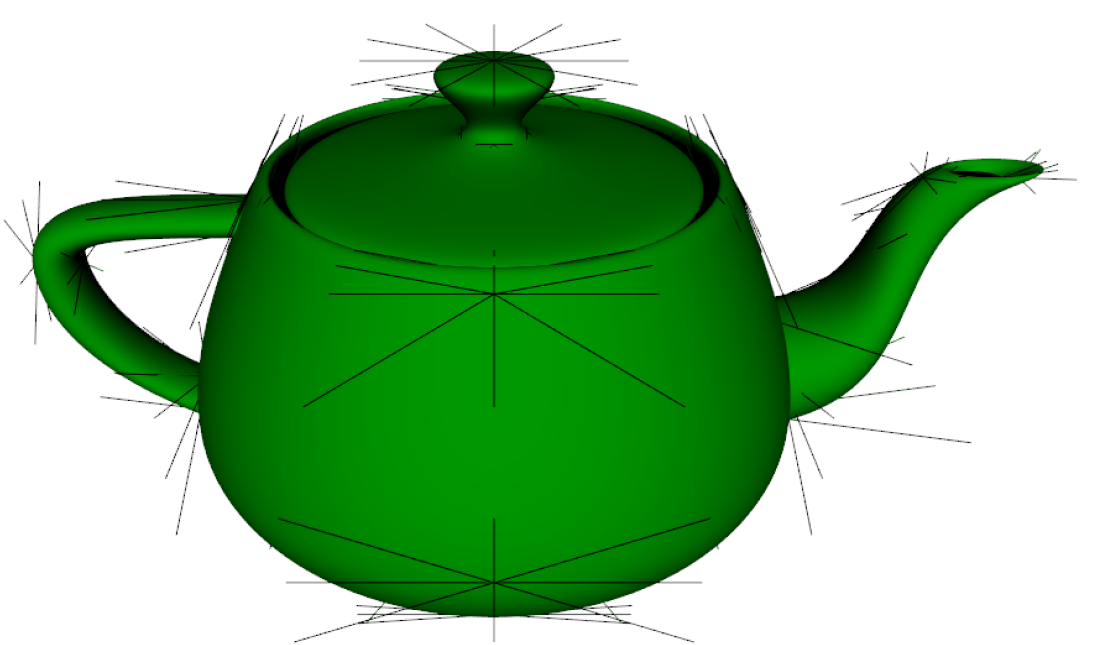
\includegraphics[width=0.5\textwidth]{testing-teapot.png}
    \caption{Тестування програми на стандартній моделі}\label{fig:testing-teapot}
\end{figure}

Інтерфейс користувача розробленої програми наведено на рис. \cite{fig:beginning-interface}

\begin{figure}[!htb]
    \centering
    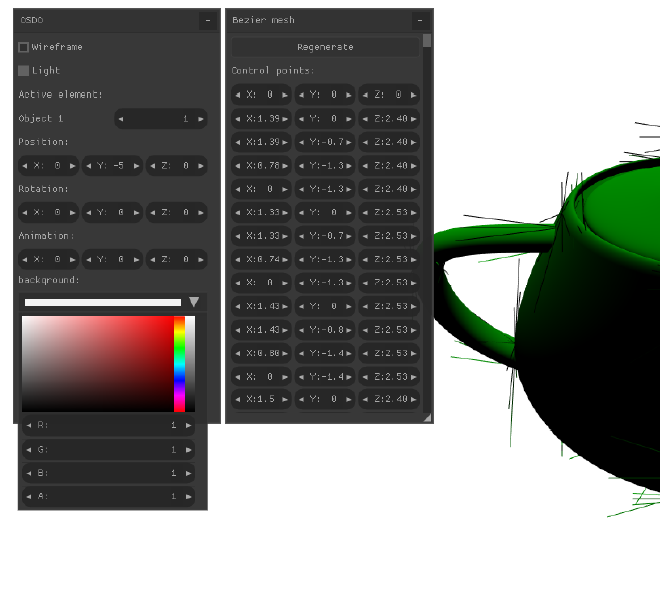
\includegraphics[width=0.5\textwidth]{beginning-interface.png}
    \caption{Інтерфейс користувача програми}\label{fig:beginning-interface}
\end{figure}

На рис. \cite{fig:teapot-wireframe} продемонстровано побудовану з використанням розробленого програмного додатку каркасну модель тестового прикладу.

\begin{figure}[!htb]
    \centering
    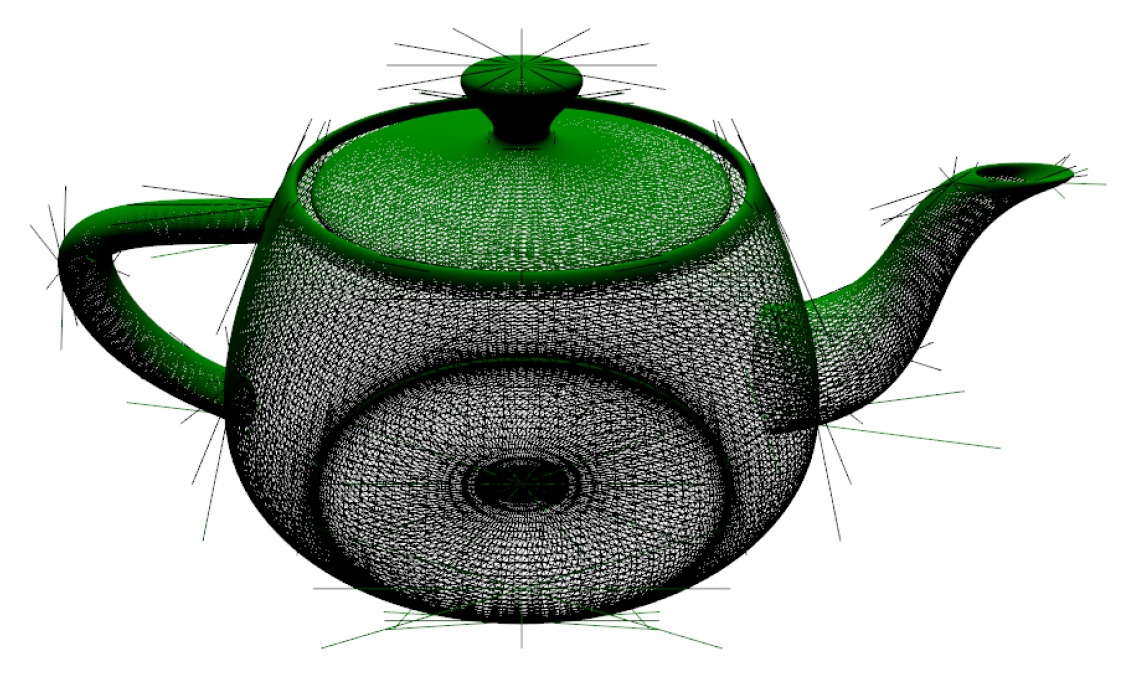
\includegraphics[width=0.5\textwidth]{teapot-wireframe.png}
    \caption{Генерація каркасної моделі тестового прикладу}\label{fig:teapot-wireframe}
\end{figure}

Далі розглянемо приклад створення об'єкту за допомогою розробленої програми. При початковому завантаженні програми ми отримаємо вікно, яке продемонстровано на рис.4. Для налаштування області виводу зображення користувач може скористуватися головним та допоміжним вікнами. У допоміжному вікні є можливість перемкнутися у режим каркасу, перемкнути режим світла. Зробивши камеру джерелом світла також можна вибрати активний елемент з наявних (за замовчанням це камера).

У активному елементі ми можемо задати позицію, поворот та анімацію повороту. Якщо перемкнутися на деякий об'єкт  отримаємо наступні екрани (рис. \cite{fig:edit-car} \cite{car-view}).

\begin{figure}[!htb]
    \centering
    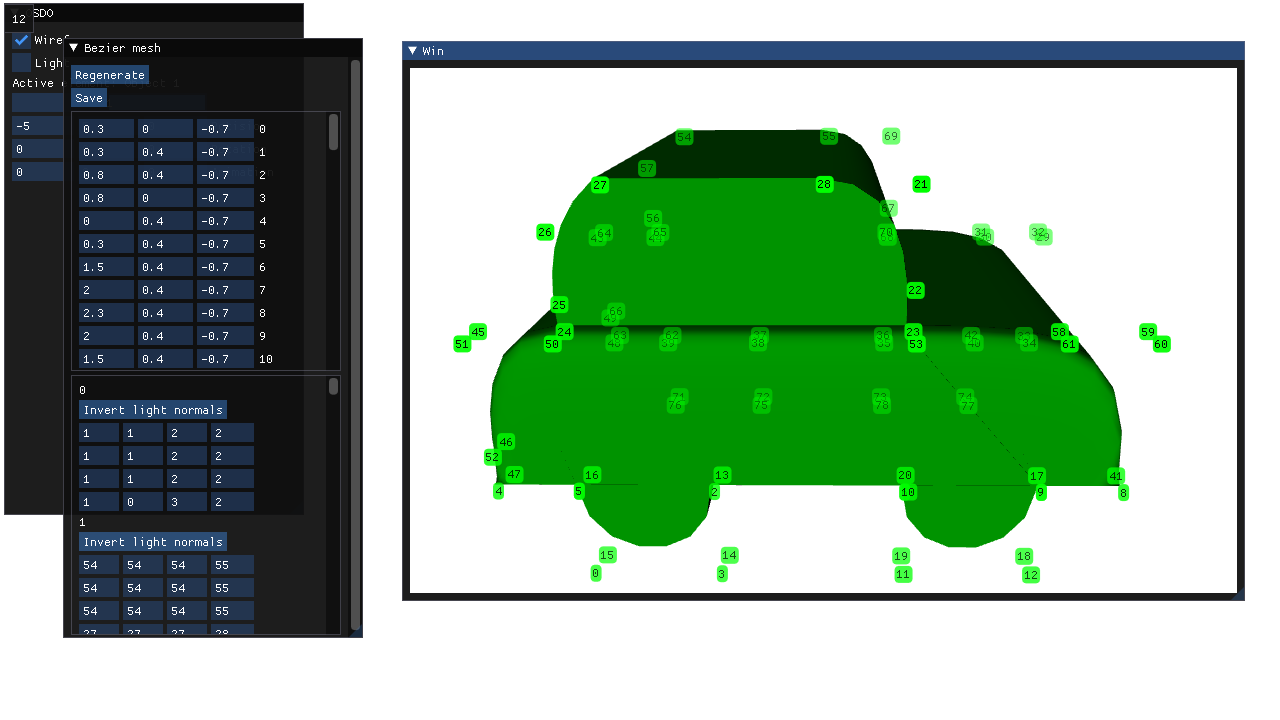
\includegraphics[width=0.5\textwidth]{edit-car.png}
    \caption{Генерація моделі (режим редагування)}\label{fig:edit-car}
\end{figure}

\begin{figure}[!htb]
    \centering
    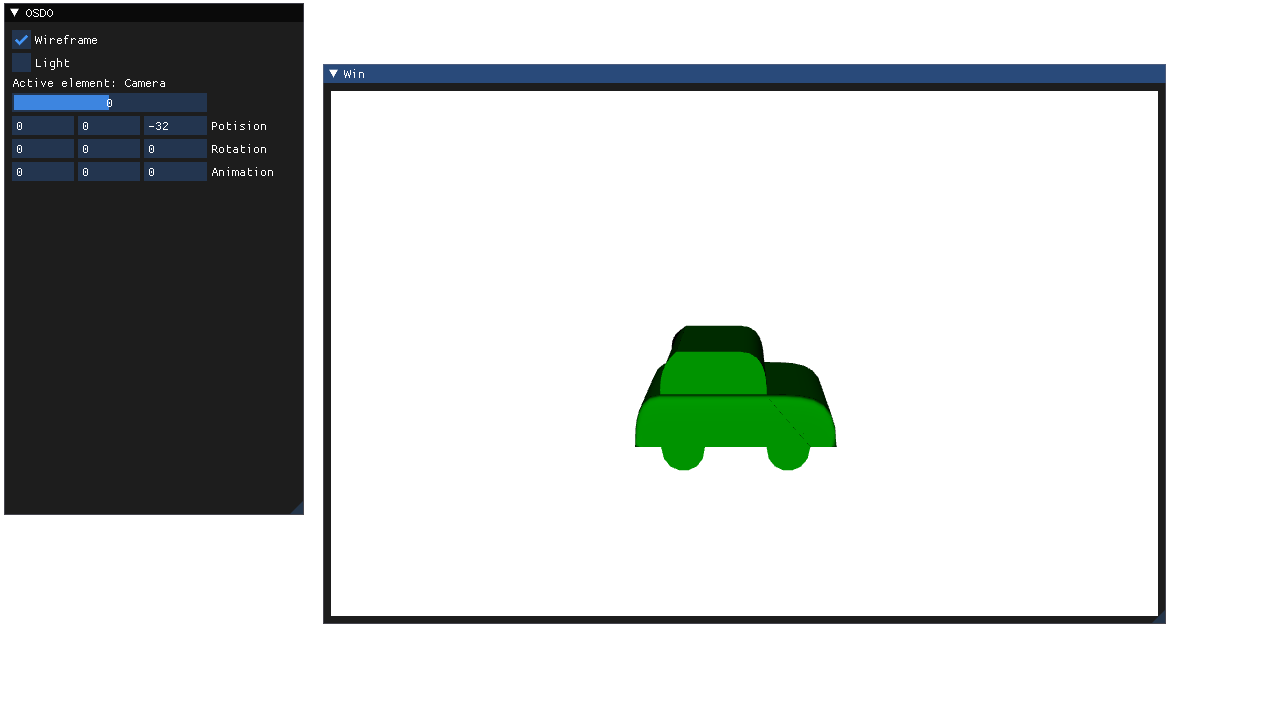
\includegraphics[width=0.5\textwidth]{car-view.png}
    \caption{Генерація моделі (режим редагування)}\label{fig:car-view}
\end{figure}

У даному режимі з'являється можливість редагування об'єкту побудованого за допомогою поверхонь Безьє. Загалом на головному вікні з'являються номери контрольних точок. Також з'являється третє вікно у якому присутні такі елементи:

\begin{itemize}
\item Кнопка "Regenerate" - дозволяє перебудувати об'єкт
\item Кнопка "Save" - зберігає об'єкт на диск
\item Підвікно з можливістю знайти контрольну точку за її номером та змінити її координати
\item Підвікно з можливістю знайти одну з поверхонь та відредагувати такими елементами:
\item Кнопка "Invert light normals" - дозволяє змінити порядок контрольних точок поверхні для того щоб нормалі поверхні дивилися в протилежну сторону.
\item 16 полів з номерами контрольних точок.
\end{itemize}

\section{Основна документація до коду}

\subsection{Алфавітний покажчик класів}
\doxysubsection{Класи}
Класи, структури, об\textquotesingle{}єднання та інтерфейси з коротким описом.\begin{DoxyCompactList}
\item\contentsline{section}{\mbox{\hyperlink{classBeziator}{Beziator}} \\*Клас який зберігає та оброблює модель утвореню через поверхні Безьє }{}{}
\item\contentsline{section}{\mbox{\hyperlink{classBijective}{Bijective}} \\*Інтерфейс до об\textquotesingle{}єктів, що можуть можуть бути переміщені та повернуті у просторі }{}{}
\item\contentsline{section}{\mbox{\hyperlink{classBuffer}{Buffer}} \\*Буфер, у якому відбувається рендеринг у текстуру }{}{}
\item\contentsline{section}{\mbox{\hyperlink{classCamera}{Camera}} \\*Клас камери, якою можна маніпулювати у сцені }{}{}
\item\contentsline{section}{\mbox{\hyperlink{structContext}{Context}} \\*Контекст, який зберігає усі завантажені у пам\textquotesingle{}ять ресурси }{}{}
\item\contentsline{section}{\mbox{\hyperlink{classFramebuffer}{Framebuffer}} \\*Буфер кадру, що використовується для рендеренгу }{}{}
\item\contentsline{section}{\mbox{\hyperlink{classGlBindable}{Gl\+Bindable}} \\*Абстрактний клас, який виконує роль генерації та прив\textquotesingle{}язки об\textquotesingle{}єктів Open\+GL }{}{}
\item\contentsline{section}{\mbox{\hyperlink{classGlBinder}{Gl\+Binder}} \\*Клас який прив\textquotesingle{}язує контексту до деякого об\textquotesingle{}єкту Open\+GL }{}{}
\item\contentsline{section}{\mbox{\hyperlink{classImage}{Image}} \\*Зберігає масив пікселів, ширину та висоту }{}{}
\item\contentsline{section}{\mbox{\hyperlink{classMesh}{Mesh}} \\*Меш, який зберігається на відеокарті }{}{}
\item\contentsline{section}{\mbox{\hyperlink{classModel}{Model}} \\*Інтерфейс до деякої моделі, яку можна відобразити }{}{}
\item\contentsline{section}{\mbox{\hyperlink{classObject}{Object}} \\*Об\textquotesingle{}єкт моделі }{}{}
\item\contentsline{section}{\mbox{\hyperlink{classRenderbuffer}{Renderbuffer}} \\*Буфер рендеренгу (для зберігання кольорів або глибини) }{}{}
\item\contentsline{section}{\mbox{\hyperlink{structScene}{Scene}} \\*Сцена із об\textquotesingle{}єктами }{}{}
\item\contentsline{section}{\mbox{\hyperlink{classShader}{Shader}} \\*Клас взаємодії з шейдером у видеокарті }{}{}
\item\contentsline{section}{\mbox{\hyperlink{classShaderSource}{Shader\+Source}} }{}{}
\item\contentsline{section}{\mbox{\hyperlink{classTexture}{Texture}} \\*Клас текстури, що зберігаэться у відеокарті }{}{}
\item\contentsline{section}{\mbox{\hyperlink{classOSDO_1_1vector}{OSDO\+::vector$<$ T $>$}} \\*Вектор що не змінює свій розмір }{}{}
\item\contentsline{section}{\mbox{\hyperlink{structVertex}{Vertex}} \\*Структура вершини, для передачі у відеокарту }{}{}
\end{DoxyCompactList}


../latex/classBeziator.tex

\section*{ВИСНОВКИ}
\addcontentsline{toc}{section}{ВИСНОВКИ}
У ході курсової роботи були отримані такі результати:

\begin{itemize}
\item розширено функціонал розробленого програмного забезпечення, розробленого у курсовій роботі, загалом додати можливість динамічно завантажувати моделі, змінювати деталізацію.
\item зроблено програмне забезпечення придатним для компіляції та роботи у різних операційних системах, загалом Linux та Windows
\item розроблено шйедер для генерації 3D-моделі за допомогою відеокарти.
\item написано документацію до програмного забезпечення.
\end{itemize}

\begin{thebibliography}{9}
\bibitem{} Офіційний сайт Міністерства освіти та науки України: http://mon.gov.ua/
\bibitem{} СТП-02066747-009-01. Стандарт Дніпропетровського національного університету. Методика виконання випускних, курсових та дипломних проектів (робіт). Структура, правила оформлення та порядок узгодження і затвердження. Затверджено ректором ДНУ 31.10.2001 р.
\bibitem{} СТП-02066747-010-01. Стандарт Дніпропетровського національного університету. Організація та проведення дипломування. Затверджено ректором ДНУ 1.11.2001 р.
\bibitem{} http://www.dnu.dp.ua/docs/obgovorennya/Polozhennya\_Antiplagiat\_2016.doc
\bibitem{porev} Порев. В.Н. Компъютерная графика -- СПб: БХВ-Петербург, 2002 -- 432 c.
\bibitem{nikulin} Никулин Е. A. Компъютерная геометрия и алгоритмы машинной графики. - СПб: БХВ-Петербург, 2003 - 560 c.
\bibitem{ryabin} Вычислительная геометрия и алгоритмы компьютерной графики. Работа с 3D-графикой средствами OpenGL: учеб. пособие / К. В. Рябинин; Перм. гос. нац. исслед. ун-т. – Пермь, 2017. – 100 с.
\end{thebibliography}

%\end{document}
\section*{Додаток A. Лістинг програми}
\addcontentsline{toc}{section}{Додаток A. Лістинг програми}
\tiny
\singlespacing
\hypertarget{beziator_8h}{}\doxysubsection{Файл osdo/beziator.h}
\label{beziator_8h}\index{osdo/beziator.h@{osdo/beziator.h}}


Клас який зберігає та оброблює модель утвореню через поверхні Безьє.  


{\ttfamily \#include $<$EASTL/string.\+h$>$}\newline
{\ttfamily \#include \char`\"{}osdo.\+h\char`\"{}}\newline
{\ttfamily \#include \char`\"{}mesh.\+h\char`\"{}}\newline
Діаграма включених заголовочних файлів для beziator.\+h\+:\nopagebreak
\begin{figure}[H]
\begin{center}
\leavevmode
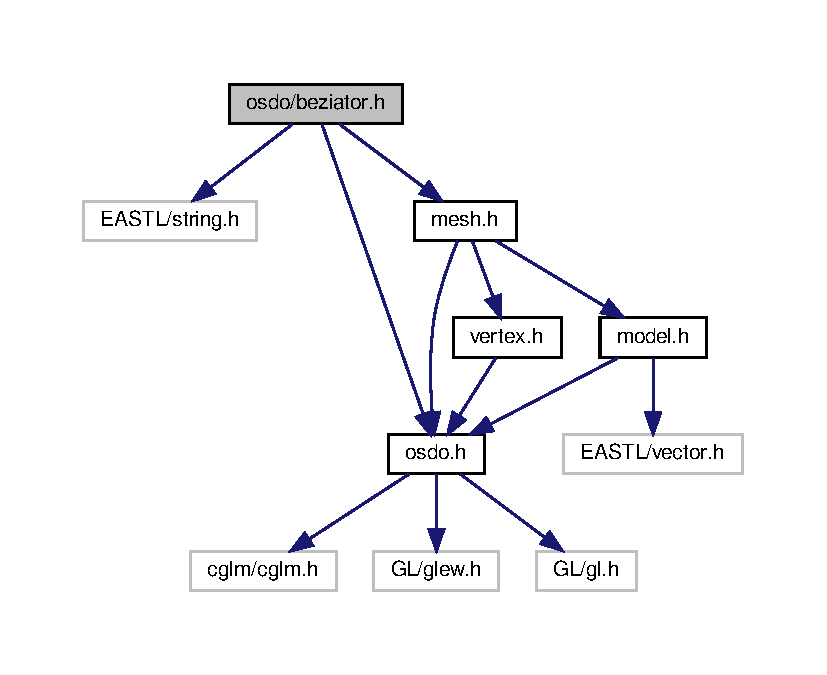
\includegraphics[width=350pt]{beziator_8h__incl}
\end{center}
\end{figure}
Граф файлів, які включають цей файл\+:\nopagebreak
\begin{figure}[H]
\begin{center}
\leavevmode
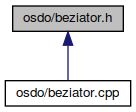
\includegraphics[width=174pt]{beziator_8h__dep__incl}
\end{center}
\end{figure}
\doxysubsubsection*{Класи}
\begin{DoxyCompactItemize}
\item 
class \mbox{\hyperlink{classBeziator}{Beziator}}
\begin{DoxyCompactList}\small\item\em Клас який зберігає та оброблює модель утвореню через поверхні Безьє. \end{DoxyCompactList}\end{DoxyCompactItemize}
\doxysubsubsection*{Визначення типів}
\begin{DoxyCompactItemize}
\item 
typedef GLuint \mbox{\hyperlink{beziator_8h_adc91dd1f882e36615956dace902ac8a2}{surfacei\+\_\+t}}\mbox{[}4\mbox{]}\mbox{[}4\mbox{]}
\begin{DoxyCompactList}\small\item\em Набір індексів на вершини, що утворюють поверхню 4x4. \end{DoxyCompactList}\end{DoxyCompactItemize}


\doxysubsubsection{Детальний опис}
Клас який зберігає та оброблює модель утвореню через поверхні Безьє. 



Див. визначення в файлі \mbox{\hyperlink{beziator_8h_source}{beziator.\+h}}



\doxysubsubsection{Опис визначень типів}
\mbox{\Hypertarget{beziator_8h_adc91dd1f882e36615956dace902ac8a2}\label{beziator_8h_adc91dd1f882e36615956dace902ac8a2}} 
\index{beziator.h@{beziator.h}!surfacei\_t@{surfacei\_t}}
\index{surfacei\_t@{surfacei\_t}!beziator.h@{beziator.h}}
\doxyparagraph{\texorpdfstring{surfacei\_t}{surfacei\_t}}
{\footnotesize\ttfamily typedef GLuint surfacei\+\_\+t\mbox{[}4\mbox{]}\mbox{[}4\mbox{]}}



Набір індексів на вершини, що утворюють поверхню 4x4. 



Див. визначення в файлі \mbox{\hyperlink{beziator_8h_source}{beziator.\+h}}, рядок \mbox{\hyperlink{beziator_8h_source_l00017}{17}}


../latex/beziator_8h_source.tex
\hypertarget{bezier_8frag}{}\doxysubsection{Файл res/bezier.frag}
\label{bezier_8frag}\index{res/bezier.frag@{res/bezier.frag}}

../latex/bezier_8frag_source.tex
../latex/bezier_8geom.tex
\hypertarget{bezier_8geom_source}{}\doxysubsection{bezier.\+geom}
\label{bezier_8geom_source}\index{res/bezier.geom@{res/bezier.geom}}

\begin{DoxyCode}{0}
\DoxyCodeLine{00001 \#version 420 core}
\DoxyCodeLine{00002 layout(triangles) in;}
\DoxyCodeLine{00003 layout(triangle\_strip, max\_vertices=16) out;}
\DoxyCodeLine{00004 }
\DoxyCodeLine{00005 struct Data \{}
\DoxyCodeLine{00006     vec4 color;}
\DoxyCodeLine{00007     vec2 uv;}
\DoxyCodeLine{00008     vec3 normal;}
\DoxyCodeLine{00009     vec3 frag\_pos;}
\DoxyCodeLine{00010 \};}
\DoxyCodeLine{00011 }
\DoxyCodeLine{00012 in Data vertex[3];}
\DoxyCodeLine{00013 out Data geometry;}
\DoxyCodeLine{00014 }
\DoxyCodeLine{00015 void main() \{}
\DoxyCodeLine{00016     int i;}
\DoxyCodeLine{00017     for(i = 0; i < 16; i++) \{}
\DoxyCodeLine{00018         gl\_Position = gl\_in[i].gl\_Position;}
\DoxyCodeLine{00019         geometry.color = vertex[i].color;}
\DoxyCodeLine{00020         geometry.uv = vertex[i].uv;}
\DoxyCodeLine{00021         geometry.pos = vertex[i].pos;}
\DoxyCodeLine{00022         geometry.normal = vertex[i].normal;}
\DoxyCodeLine{00023         EmitVertex();}
\DoxyCodeLine{00024     \}}
\DoxyCodeLine{00025     EndPrimitive();}
\DoxyCodeLine{00026 \}}

\end{DoxyCode}

../latex/bezier_8tesc.tex
../latex/bezier_8tesc_source.tex
\hypertarget{bezier_8tese}{}\doxysubsection{Файл res/bezier.tese}
\label{bezier_8tese}\index{res/bezier.tese@{res/bezier.tese}}

\hypertarget{bezier_8tese_source}{}{bezier.\+tese}
\label{bezier_8tese_source}\index{res/bezier.tese@{res/bezier.tese}}

\begin{DoxyCode}{0}
\DoxyCodeLine{00001 \#version 420 core}
\DoxyCodeLine{00002 }
\DoxyCodeLine{00003 layout(quads, equal\_spacing) in;}
\DoxyCodeLine{00004 }
\DoxyCodeLine{00005 struct Data \{}
\DoxyCodeLine{00006     vec4 color;}
\DoxyCodeLine{00007     vec2 uv;}
\DoxyCodeLine{00008     vec3 normal;}
\DoxyCodeLine{00009     vec3 frag\_pos;}
\DoxyCodeLine{00010 \};}
\DoxyCodeLine{00011 }
\DoxyCodeLine{00012 layout(location = 0) in Data inData[];}
\DoxyCodeLine{00013 layout(location = 0) out Data outData;}
\DoxyCodeLine{00014 }
\DoxyCodeLine{00015 mat4  b = mat4 ( 1,  0,  0, 0,}
\DoxyCodeLine{00016                 -\/3,  3,  0, 0,}
\DoxyCodeLine{00017                  3, -\/6,  3, 0,}
\DoxyCodeLine{00018                 -\/1,  3, -\/3, 1);}
\DoxyCodeLine{00019 }
\DoxyCodeLine{00020 void main(void) \{}
\DoxyCodeLine{00021     float x = gl\_TessCoord.x;}
\DoxyCodeLine{00022     float y = gl\_TessCoord.y;}
\DoxyCodeLine{00023     vec4 u = vec4 (1.0, x, x*x, x*x*x);}
\DoxyCodeLine{00024     vec4 v = vec4 (1.0, y, y*y, y*y*y);}
\DoxyCodeLine{00025     vec4 uu = vec4 (0, 1.0, 2*x, 3*x*x);}
\DoxyCodeLine{00026     vec4 vv = vec4 (0, 1.0, 2*y, 3*y*y);}
\DoxyCodeLine{00027 }
\DoxyCodeLine{00028     vec4 bu = b * u;}
\DoxyCodeLine{00029     vec4 bv = b * v;}
\DoxyCodeLine{00030     vec4 buu = b * uu;}
\DoxyCodeLine{00031     vec4 bvv = b * vv;}
\DoxyCodeLine{00032 }
\DoxyCodeLine{00033     mat4 pu[4], pv[4], cu, cv;}
\DoxyCodeLine{00034     for (int i = 0; i < 4; i++) \{}
\DoxyCodeLine{00035         for (int j = 0; j < 4; j++) \{}
\DoxyCodeLine{00036             pv[i][j] = gl\_in[j*4 + i].gl\_Position;}
\DoxyCodeLine{00037         \}}
\DoxyCodeLine{00038     \}}
\DoxyCodeLine{00039     for (int i = 0; i < 4; i++) \{}
\DoxyCodeLine{00040         cv[i] = pv[i] * bv;}
\DoxyCodeLine{00041     \}}
\DoxyCodeLine{00042 }
\DoxyCodeLine{00043     gl\_Position = cv * bu;}
\DoxyCodeLine{00044 }
\DoxyCodeLine{00045     for (int i = 0; i < 4; i++) \{}
\DoxyCodeLine{00046         for (int j = 0; j < 4; j++) \{}
\DoxyCodeLine{00047             pu[i][j] = vec4(inData[i*4 + j].normal, 1);}
\DoxyCodeLine{00048             pv[i][j] = vec4(inData[j*4 + i].normal, 1);}
\DoxyCodeLine{00049         \}}
\DoxyCodeLine{00050     \}}
\DoxyCodeLine{00051     for (int i = 0; i < 4; i++) \{}
\DoxyCodeLine{00052         cu[i] = pu[i] * bu;}
\DoxyCodeLine{00053         cv[i] = pv[i] * bv;}
\DoxyCodeLine{00054     \}}
\DoxyCodeLine{00055     vec4 du = cv * buu, dv = cu * bvv;}
\DoxyCodeLine{00056     outData.normal = cross(vec3(du), vec3(dv));}
\DoxyCodeLine{00057 }
\DoxyCodeLine{00058     for (int i = 0; i < 4; i++) \{}
\DoxyCodeLine{00059         for (int j = 0; j < 4; j++) \{}
\DoxyCodeLine{00060             pv[i][j] = vec4(inData[j*4 + i].frag\_pos, 1);}
\DoxyCodeLine{00061         \}}
\DoxyCodeLine{00062     \}}
\DoxyCodeLine{00063     for (int i = 0; i < 4; i++) \{}
\DoxyCodeLine{00064         cv[i] = pv[i] * bv;}
\DoxyCodeLine{00065     \}}
\DoxyCodeLine{00066     outData.frag\_pos = vec3(cv * bu);}
\DoxyCodeLine{00067 }
\DoxyCodeLine{00068 }
\DoxyCodeLine{00069     /*for (int i = 0; i < 4; i++) \{}
\DoxyCodeLine{00070         for (int j = 0; j < 4; j++) \{}
\DoxyCodeLine{00071             pv[i][j] = vec4(inData[i*4 + i].uv, 0, 1);}
\DoxyCodeLine{00072         \}}
\DoxyCodeLine{00073     \}}
\DoxyCodeLine{00074     for (int i = 0; i < 4; i++) \{}
\DoxyCodeLine{00075         cv[i] = pv[i] * bv;}
\DoxyCodeLine{00076     \}}
\DoxyCodeLine{00077     outData.uv = vec2(cv * bu);*/}
\DoxyCodeLine{00078     outData.uv = vec2(x, y);}
\DoxyCodeLine{00079 }
\DoxyCodeLine{00080     outData.color = inData[0].color;}
\DoxyCodeLine{00081 \}}

\end{DoxyCode}

\hypertarget{bezier_8vert}{}\doxysubsection{Файл res/bezier.vert}
\label{bezier_8vert}\index{res/bezier.vert@{res/bezier.vert}}

../latex/bezier_8vert_source.tex

\end{document}
